\documentclass[a4paper,12pt]{report}
\usepackage[polish]{babel}
\usepackage[utf8]{inputenc}
\usepackage[T1]{fontenc}
\usepackage{geometry}
\usepackage{enumitem}
\usepackage{graphicx}
\usepackage{float}
\usepackage{minted}

\usepackage{xcolor} % to access the named colour LightGray
\definecolor{LightGray}{gray}{0.9}

\graphicspath{{./images/}}

\selectlanguage{polish}

\geometry{
    left=20mm, 
    right=20mm, 
    top=20mm,
    bottom=20mm
}

\definecolor{my-bg}{rgb}{0.95,0.95,0.95}
\setminted[python]{
    breaklines=true,
    mathescape=true,
    linenos=true,
    numbersep=5pt,
    bgcolor=my-bg
}

\title{Praca Inżynierska\\{\Large Politechnika Śląska}}
\author{Szymon Ciemała}
\date{Październik 2021}

\begin{document}

\maketitle

\tableofcontents

\chapter{Wstęp}
\begin{itemize}
\item wprowadzenie w problem/zagadnienie
\item osadzenie problemu w dziedzinie
\item cel pracy
\item zakres pracy
\item zwięzła charakterystyka rozdziałów
\item jednoznaczne określenie wkładu autora, w przypadku prac wieloosobowych – tabela z autorstwem poszczególnych elementów pracy
\end{itemize}

\newpage

\section{Wprowawdzenie w problem}
\quad Rozwój technolgii w ostatnich czasach przyczynił się do coraz częstszego wykorzystywania wizji komputerowej oraz metod uczenia maszynowego do rozpoznawania oraz klasyfikacji różnego typu obiektów, w tym części ludzkiego ciała. Pozwala to na interakcję człowieka z aplikacjami, często w spób bardziej naturalny. 

\section{Cel pracy}
Projekt inżynierski ma na celu stworzenie biblioteki w języku Python, która pozwoli na przystępne wykorzystanie algorytmów rozpoznawania gestów oraz ruchu dłoni. Biblioteka powinna oferować gotowe rozwiązania, na przykład przygotowane modele matematyczne pozwalające na rozpoznawanie języka migowego oraz gestów podstawowych. Dodatkowo powinna pozowlić na wyznaczenie pozycji dłoni, jej typu oraz wartości charakterystycznych, na przykład odlgłości między końcówkami wybranych palców czy kąta obrotu dłoni. 

\section{Osadzenie problemu w dziedzienie}
\quad Aktualnie istnieją częściowo gotowe rozwiązania pozwalające na rozpoznanie i klasyfikację dłoni - bibliotka MediaPipe. 

\section {Charakterystyka rozdziałów}

\quad W pierwszym rozdziale zostanie poruszony temat genezy problemu oraz jego sformułowania. Zostaną dodatkowo opisane jego założenia wraz z wyamaganą funkcjonalnością projektu. 

\quad W drugim temacie zostaną opisne techniczne tworzonej biblioteki oraz narzędzia wymagane do jej stworzenia. Zakres opisywanych narzędzi rozpocznie się od opisu wybranego systemu operacyjnego do programów służących do stworzenia pobieralnej paczki na platformi PyPi.

\quad W rozdziale nr 5 zostaną opisane wymagania sprzętowe wymagane do poprawnego działania funkcji biblioteki. Przedstawione zostanie działanie klasy wraz z jej parametrami oraz sposób jego wykorzysania. W drugiej jego części zostaną przedstawione przykłady wykorzysania modułu. Przykładowym projektami będą: program rozpoznający gest, interaktywny kiosk bezdotykowy i system doboru koloru przy pomocy gestu. 

\quad Kolejny rozdział opisuje budowę klasy wraz z najważniejszymi algorytmami oraz strukturami danych. Dodakowo opisany zostanie Jupyter Notebook służący do generowania modeli uczenia maszynowego rozpoznających gest dłoni. 

% \section{Ogólnie}

% Praca przedstawia wykorzystanie bibliotek OpenCV, MediaPipe oraz metod 
% uczenia maszynowego bibliteki SciKit Learn do stworzenia modułu dla 
% języka Python, który umożliwi sterwowanie dowolnymi aplikacjami przy 
% użyciu gestów oraz ruchu dłońmi. 

% \section{Wykorzystane technologie}
% \subsection{OpenCV}
% Biblioteka, dzieki której można wykorzystać obraz z kamery oraz wstępnie
% przetworzyć obraz, który zostanie wykorzystany przez bibliotekę MediaPipe.

% \subsection{MediaPipe}

% \quad
% Biblioteka MediaPipe o otwartym źródle, udostępnia wieloplatformowe oraz 
% konfigurowalne rozwiązania wykrzustujące uczenie maszynowe w dziedzienie 
% rozpoznawania, segmentacji oraz klasyfikacji obiektów wizji komputerowej. 
% Niektórymi z rozwiązań są:

% \begin{itemize}
%     \item Rozpoznawanie twarzy
%     \item Segmentacjia włosów oraz twarzy
%     \item Rozpoznawnie oraz określanie rozmiarów obiektów trójwymiarowych na podstawie obrazu dwuwymiarowego. 
% \end{itemize}

% Platformy/Języki programowania obsługiwane przez MediaPipe:

% \begin{itemize}
%     \item Android
%     \item IOS
%     \item JavaScript
%     \item Python
%     \item C++
%     \item Coral
% \end{itemize}

% ????
% Pozwoli na rozpoznaie dłoni oraz jej elementów charakterystycznych, 
% takich jak nagdarstek, stawy oraz końcówki palców. 
% ???


% \subsection{SciKit Learn}

% SciKit Learn to biblioteka, która oferuje różnego typu metody uczenia
% maszynowego. Biblioteka zawiera algorytmy klasyfikacji, regresjii oraz 
% analizy skupień. 
% Biblioteka pozwala na wykorzystanie metod klasyfikacji uczenia maszynowego. 
% Co pozwli na rozpoznanie gestów dłoni. 


\chapter{Założenia projektowe}

\section{Budowa modułu}
Moduł został napisany przy pomocy paradygmatu programowania
obiektowego, co pozwala na przystępne wykorzystanie biblioteki w dowonych 
projektach wymagających osbługi gestów. 

\section{Dostęp}
Całość projektu będzie dostępna na platformie GitHub wraz z możliwością 
pobrania przy pomocy programu pip ze zdlanego repozytorium PyPi, dzięki czemu 
pozowli to na sprawne i proste wykorzystanie modułu w dowolnym 
projekcie. 

\chapter{Część techniczna/praktyczna}
\section{Rozpoznawanie dłoni}

\quad Pierwszym elementem projektu jest rozpoznanie dłoni poprzez wyznacznie pozycji elementów charakterystycznych. Pozycja każdego z tych elementów jest względna wedłgu pozycji nadgarstka. ????



\subsection{Elementy charakterystyczne}

\quad Model modułu MediaPipe pozwala na wyznaczenie pozycji 21 elementów charakterystycznych dłoni. Współrzędne X i Y są znomralizowane względem rozdzielczości obrazu kamery. Współrzędna X względem liczby pikseli w osi X, a współrzędna Y względem liczby pikseli w osi Y. Oś Z jest prostopadła do osi X i Y, z punktem początkowym w punkcie określającym pozycję nadgarstka. Współrzędna Z jest znormalizowana względem szerokości obrazu kamery, tak jak współrzędna X. 

\begin{figure}[H]
\begin{center}
    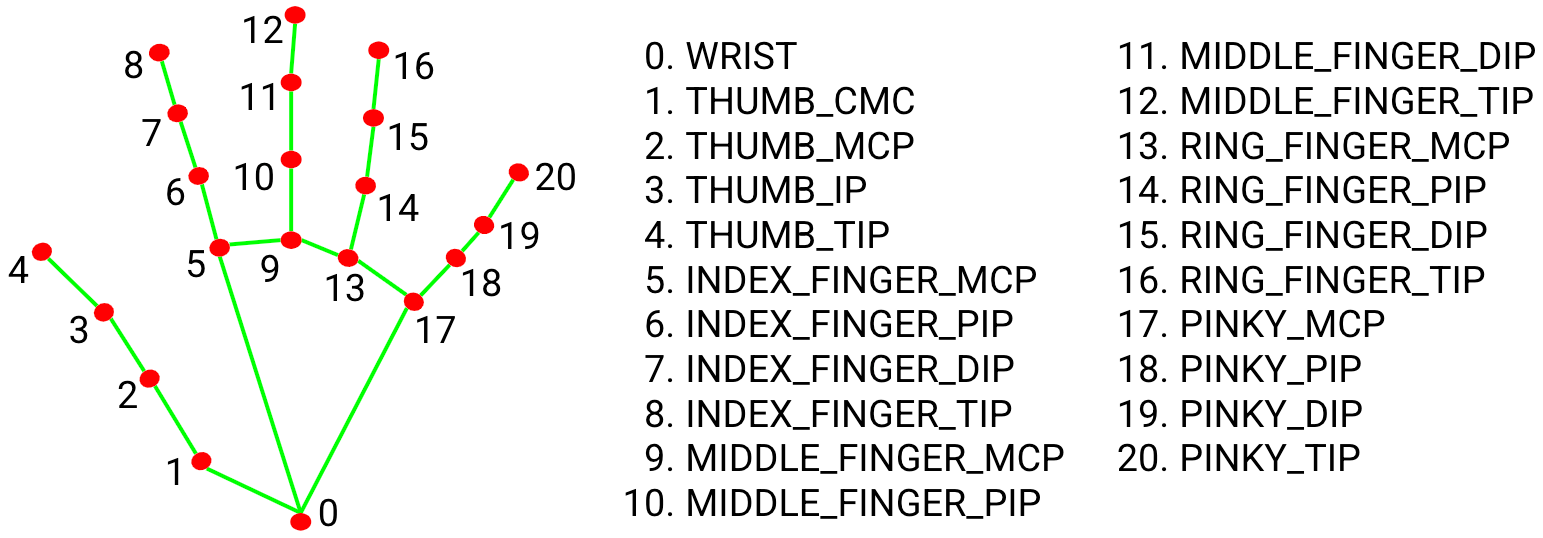
\includegraphics[width=15cm]{hand_landmarks.png}
    \caption{Elementy charakterystyczne dłoni}
\end{center}
\end{figure}

\quad Pozycje nadgarstka, paliczków oraz stawów dłoni zostaną wykorzystane do obliczenia obrotu dłoni względem punkut 0 oraz do wytrenowania modeli uczenia maszynowego, których zadaniem będzie rozpoznawnie wybranych gestów. 

\newpage
\subsection{OpenCV - przygotowanie obrazu z kamery}

\quad Poprawne działanie modelu MediaPipe wymaga odpowiedniego przygotowania obrazu kamery. Działanie kontrolerolera odbywa się poprzez główną metodę \textbf{main()}.

Metoda \textbf{main()} jest główną funkcją, w której dokonywane są obliczenia oraz przeszktałcenia pozwalające na obliczenie obrotu dłonie, odległości między wybranymi palcami oraz na wykrycie gestu. 

\inputminted[firstline=51, lastline=52]{python}{../OpenLeap.py}

\quad W pierwszym kroku tworzymy instancję klasy \textbf{VideoCapture} biblioteki \textbf{OpenCV}, która pozwoli na odczytywanie obrazu kamery. 

\inputminted[firstline=272, lastline=297]{python}{../OpenLeap.py}


\quad tekst testowy

\subsection{Generowanie grafiki dłoni}

\section{SciKit Learn - uczenie maszynowe}
\subsection{Budowa programu}
\subsection{Zebranie danych}
\subsection{Metody klasyfikacji - uczenie maszynowe}
\subsection{Ponowne wykorzystanie modelu}

\section{Paczka PyPi}
\subsection{Budowa paczki}
\subsection{Plik setup.py}
\subsection{Załadowanie paczki do repozytorium}


\chapter{Możliwości wykorzystania}
\section{Kioski samoobsługowe}
\section{Obsługa komputera}
\section{Sterowanie Robotami Mobilnymi}

\end{document}